%\documentstyle [12pt]{aastex}
\documentclass[10pt,preprint]{aastex} 
%\documentclass[11pt,preprint]{aastex} 
%\documentclass[iop,apj,tighten]{emulateapj}
%\documentclass{emulateapj}
%\usepackage{apjfonts}
%\usepackage{lineno}
%\usepackage{natbib}
\usepackage{epsf}
\usepackage{url}
\usepackage{color}
\usepackage{mathrsfs, amsmath}

%\usepackage[plainpages=false, colorlinks=true, anchorcolor=blue,
%linkcolor=blue, citecolor=blue, bookmarks=false]{hyperref}
%\citestyle{apj}

%\newcommand{\qus}   {\section*}
%\newcommand{\r}{\rho}
\newcommand{\Msun}{\ifmmode\mbox{M}_{\odot}\else$\mbox{M}_{\odot}$\fi\,}
\newcommand{\f}{\frac}
\newcommand{\D}{{\bf \nabla}}
\newcommand{\cross}{\times}
\newcommand{\dotp}{{\bf \cdot}} \setlength{\textwidth}{15cm} \setlength{\textheight}{24.0cm}
\setlength{\topmargin}{0.0cm}
\setlength{\leftmargin}{0.0cm}
\setlength{\topskip}{0.0cm}
\setlength{\headheight}{0.5cm}
\setlength{\headsep}{0.0cm}
\setlength{\oddsidemargin}{0.0cm}
\setlength{\evensidemargin}{0.0cm}
\flushbottom

%\include{graphic}
%\include{graphicx}
\begin{document}
%\title{ Understanding the origin of eccentric millisecond pulsar binaries}
%\author{Weiwei Zhu, Paulo Freire and the PALFA Consortium}
%\maketitle
%\date

\include{"partable"}

\begin{figure}
    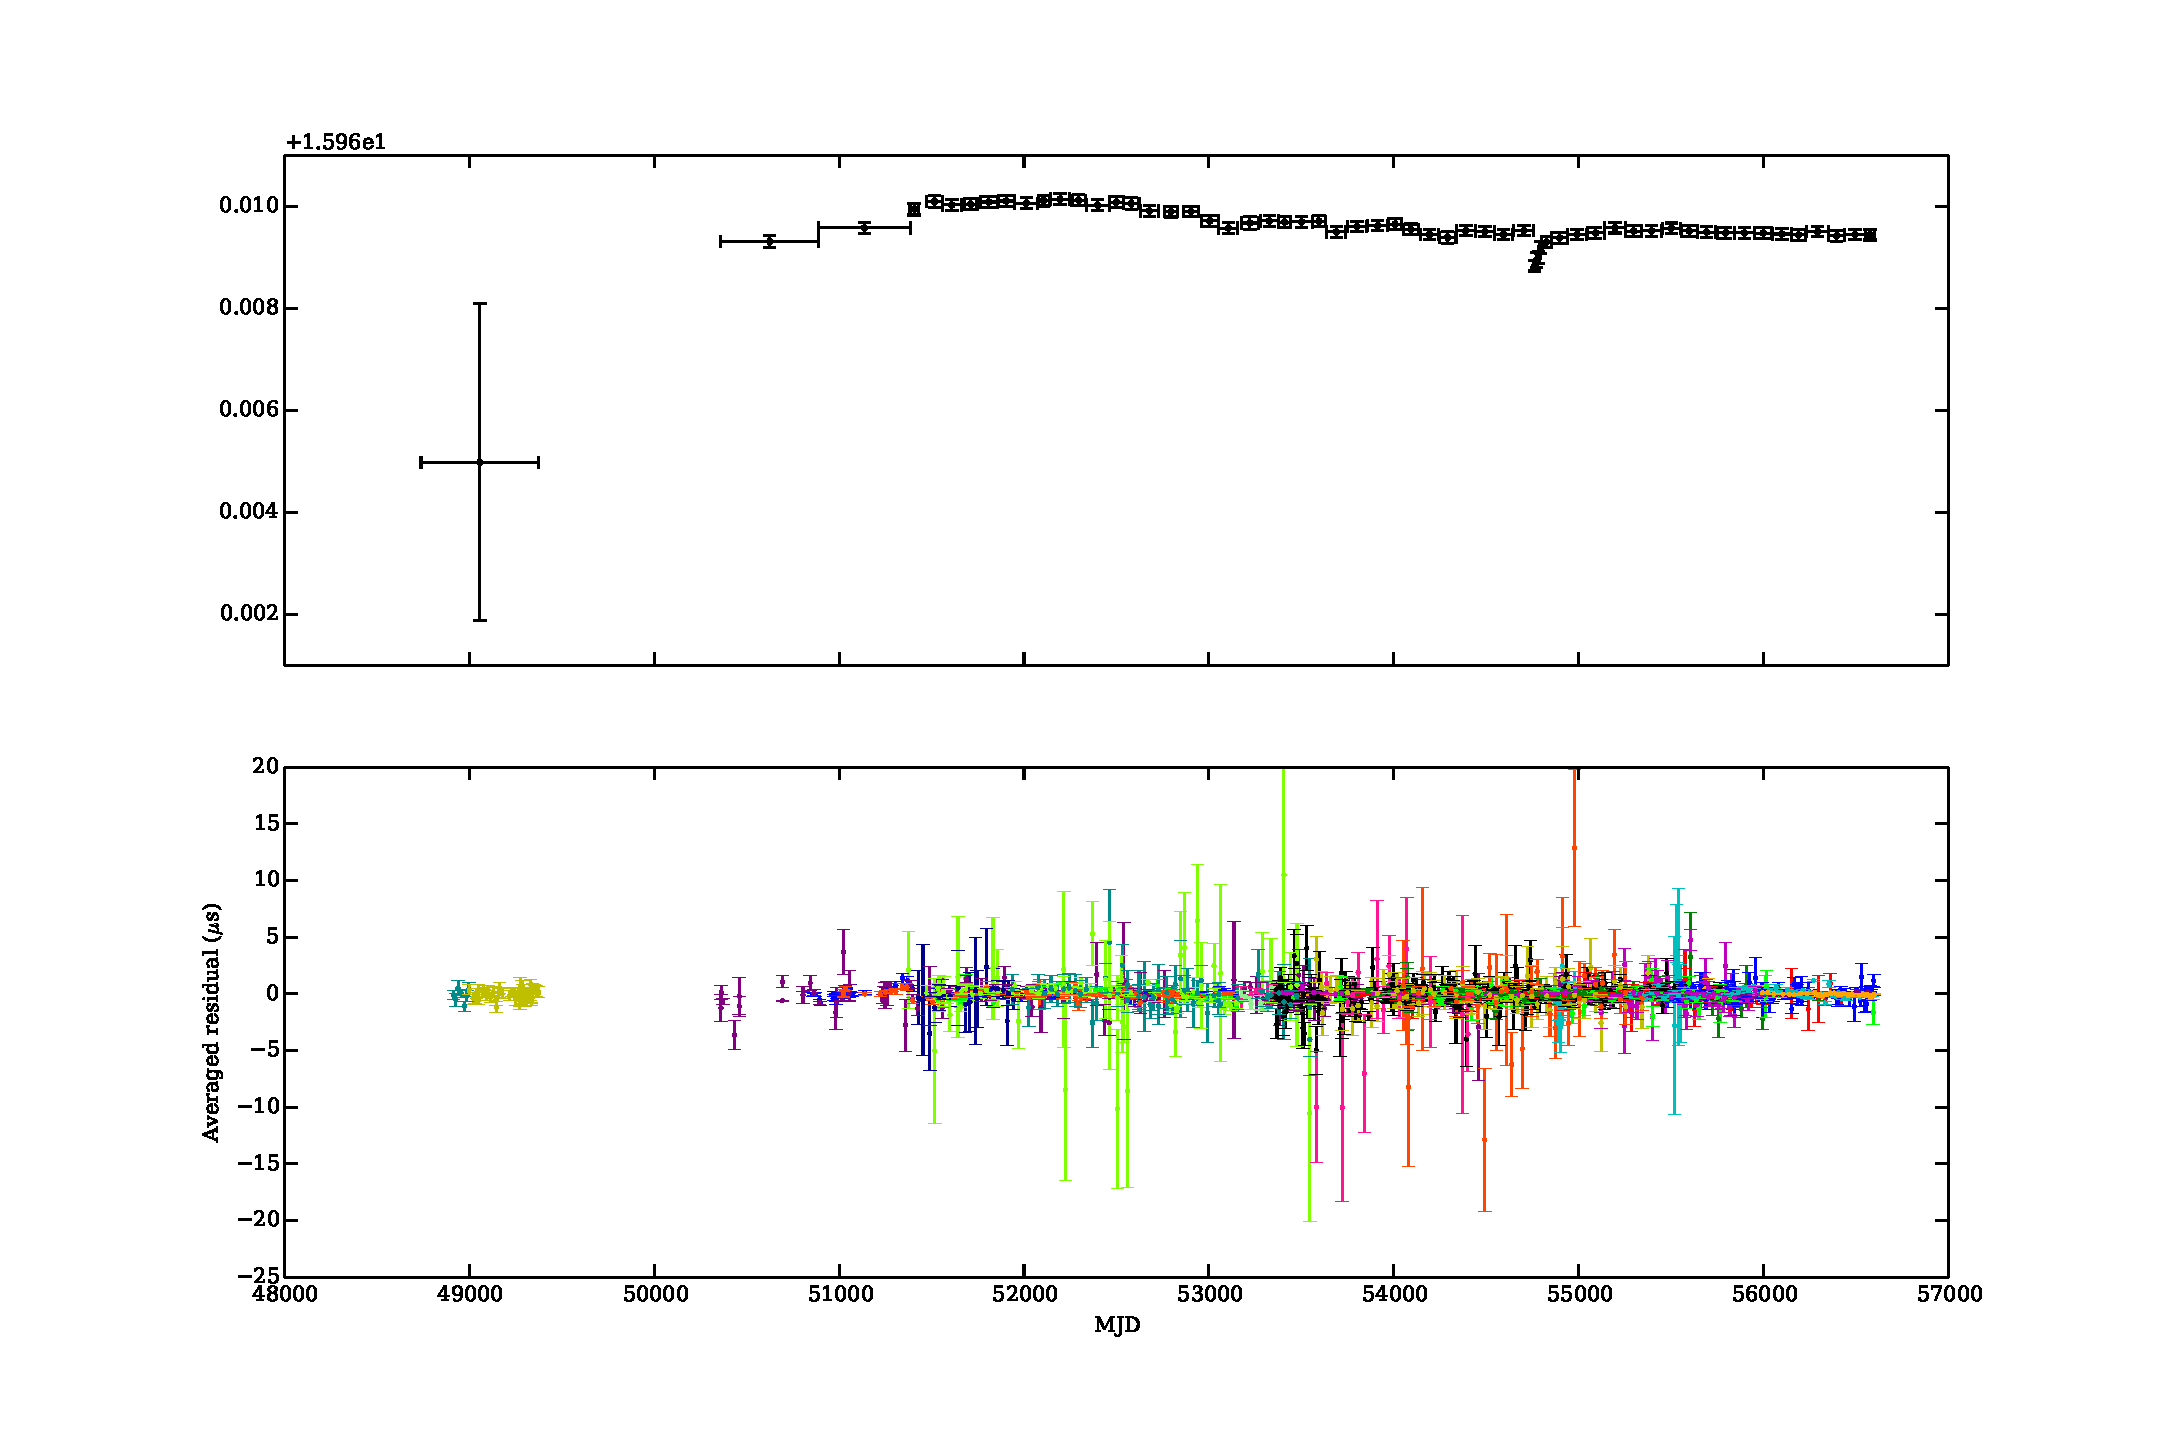
\includegraphics[width=14cm]{1713_dmxres.eps} \\ 
    %\caption {\label{fig:} } 
\end{figure} 


\begin{figure}
    \includegraphics[width=5cm]{1713_alpha3.ps} \\ 
    %\caption {\label{fig:} } 
\end{figure} 


\begin{figure}
    \includegraphics[width=5cm]{1713_delta.ps} \\ 
    %\caption {\label{fig:} } 
\end{figure} 

\begin{figure}
    \includegraphics[width=8cm]{1713_Gdot.ps} \\ 
    %\caption {\label{fig:} } 
\end{figure} 

\end{document}
